\chapter{Constantes d'équilibre et déplacements}\label{ch:b2:equilibrium-shifts}

Une usine d'ammoniac fait fonctionner son convertisseur vers \qty{450}{\celsius} et
\qty{200}{bar}. À température ambiante, l'équilibre \ce{N2 + 3H2 <=>
2NH3} est si déplacé vers l'ammoniac qu'un mélange des éléments pourrait en
principe être presque entièrement converti~; et pourtant les ingénieurs le chauffent, ce qui
fait reculer l'équilibre, puis le compriment à deux cents
atmosphères, ce qui coûte beaucoup d'énergie. Les raisons tiennent à un
compromis entre le point jusqu'où une réaction peut aller et la vitesse à laquelle elle y va. Ce
chapitre transforme l'\omterm{def:b2:reaction-free-energy:gibbs-energy}{enthalpie libre} des chapitres précédents en la
constante d'équilibre du volume de première année, montre comment cette constante varie
avec la température, dénombre les conditions qu'un expérimentateur peut choisir
librement, et prévoit dans quel sens un équilibre se déplace lorsqu'on modifie la
température, la pression ou la composition.

\begin{recall}
\Cref{ch:b2:reaction-free-energy}~: le critère d'évolution $\Delta_r G\,\dd\xi
\leq 0$ et la relation de Gibbs--Helmholtz~;
\cref{ch:b2:chemical-potential}~: $\Delta_r G = \Delta_r G^\circ + RT\ln Q$.
Le volume de première année~: le quotient $Q = \prod_i a_i^{\nu_i}$, la constante
d'équilibre standard $K^\circ$ comme valeur de $Q$ à l'équilibre, la loi
d'action des masses et la règle «~$Q < K^\circ$~: sens direct~», toutes énoncées alors comme
des lois~; les tableaux d'avancement~; les états finals d'une ou deux réactions. Il avait aussi
promis que le choix de la température et de la pression pour l'ammoniac et pour le
trioxyde de soufre serait expliqué ici.
\end{recall}

\begin{omfigure}
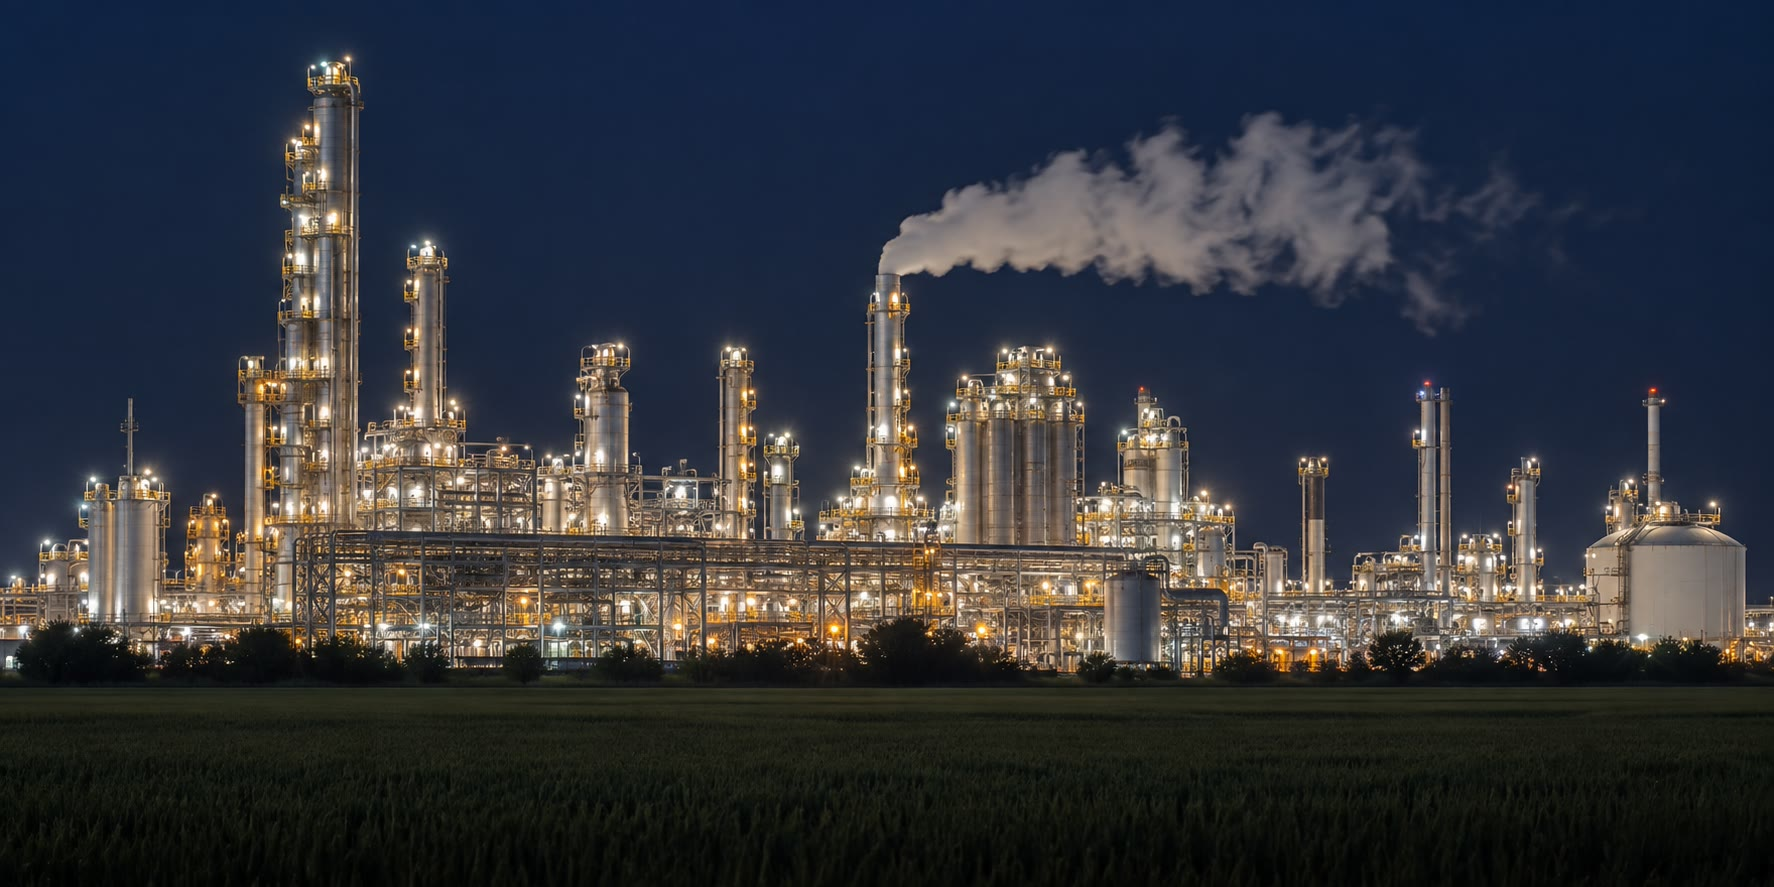
\includegraphics[width=0.7\linewidth]{images/book3/ai/b2-04-ammonia-plant.jpg}

{\small Une usine d'ammoniac la nuit. Dans son convertisseur, le diazote et le dihydrogène
passent sur un catalyseur au fer à quelques centaines de degrés et quelques centaines de bars~;
le choix de ces conditions est l'objet du problème du week-end.}
\end{omfigure}

\section{La constante d'équilibre à partir de l'enthalpie libre}

\begin{theorem}[Constante d'équilibre standard]\label{thm:b2:equilibrium-shifts:k-from-g}
À l'équilibre, $\Delta_r G = 0$, et le quotient de réaction prend la valeur
\[
  K^\circ(T) = \exp\!\left(-\frac{\Delta_r G^\circ(T)}{RT}\right), \qquad
  \Delta_r G^\circ(T) = -RT\ln K^\circ(T) .
\]
Elle ne dépend que de la température.
\end{theorem}

\begin{proof}
Le critère d'évolution fait de $\Delta_r G = 0$ la condition d'équilibre.
Avec $\Delta_r G = \Delta_r G^\circ + RT\ln Q$
(\cref{prop:b2:chemical-potential:delta-g-q}), l'équilibre signifie $\ln Q_{\text{éq}}
= -\Delta_r G^\circ/(RT)$, fonction de $T$ seule puisque $\Delta_r G^\circ$ l'est.
\end{proof}

\begin{corollary}[Les lois du volume de première année]\label{cor:b2:equilibrium-shifts:mass-action}
$\Delta_r G = RT\ln(Q/K^\circ)$. Par conséquent, un système où $Q < K^\circ$ évolue
dans le sens direct, un système où $Q > K^\circ$ dans le sens inverse, et un système où $Q = K^\circ$ est à
l'équilibre (loi d'action des masses).
\end{corollary}

\begin{proof}
Reporter $\Delta_r G^\circ = -RT\ln K^\circ$ dans $\Delta_r G = \Delta_r G^\circ
+ RT\ln Q$~; le signe de $\Delta_r G$ est celui de $\ln(Q/K^\circ)$, et le
critère d'évolution impose $\Delta_r G\,\dd\xi \leq 0$.
\end{proof}

\begin{example}[Trois constantes à \qty{298}{K}]\label{ex:b2:equilibrium-shifts:constants}
Synthèse de l'ammoniac, $\Delta_r G^\circ = \qty{-32.8}{kJ/mol}$~: $K^\circ =
\exp(32\,800/(8.314 \times 298.15)) = \num{5.6e5}$ (les tables, avec plus de
chiffres, donnent \num{5.4e5}). Dissociation de \ce{N2O4}, $\Delta_r G^\circ =
\qty{+4.7}{kJ/mol}$~: $K^\circ = 0.15$. Décomposition du calcaire,
$\Delta_r G^\circ = \qty{+130.4}{kJ/mol}$~: $K^\circ = \num{1.5e-23}$, et la
pression d'équilibre du dioxyde de carbone au-dessus du calcaire à température ambiante
vaut $\num{1.5e-23}$ bar, autant dire rien. Une variation de \qty{5.7}{kJ/mol} de
$\Delta_r G^\circ$ à \qty{298}{K} multiplie ou divise $K^\circ$ par dix.
% ledger: dfh:NH3_g, s0:NH3_g, janafG:NH3.298.15 (computed in figdata/bachelor-2/thermo-data.py and vant-hoff.py)
\end{example}

L'\omterm{def:b2:reaction-free-energy:gibbs-energy}{enthalpie libre} du système entier montre la même chose sous forme de paysage~:
elle est minimale à l'avancement d'équilibre, où sa pente, $\Delta_r G$, est
nulle.

\begin{omfigure}
\begin{tikzpicture}
\begin{axis}[
  width=0.7\linewidth, height=5.6cm, xmin=0, xmax=1, ymin=-2.2, ymax=5.2,
  axis x line=bottom, axis y line=left, xlabel={avancement $\xi$ (mol)},
  ylabel={$G(\xi) - G(0)$ (\unit{kJ})},
  tick label style={font=\small}, label style={font=\small}, clip=false]
\addplot[omDef, very thick] table[x=xi, y=G] {figdata/out/bachelor-2-gibbs-extent.dat};
\draw[dotted] (axis cs:0.189,-2.2) -- (axis cs:0.189,-0.949);
\fill[omThm] (axis cs:0.189,-0.949) circle (1.6pt);
\node[omThm, anchor=west, font=\small] at (axis cs:0.21,-1.75) {équilibre, $\xi = 0.189$};
\draw[dashed, gray] (axis cs:0,0) -- (axis cs:1,4.728);
\node[gray, font=\scriptsize, anchor=south east] at (axis cs:1,4.75) {$\xi\,\Delta_r G^\circ$};
\end{axis}
\end{tikzpicture}

{\small \omterm{def:b2:reaction-free-energy:gibbs-energy}{Enthalpie libre} d'un système fermé de gaz parfaits à \qty{298}{K} et
\qty{1}{bar}, à partir de \qty{1}{mol} de \ce{N2O4}, en fonction de l'avancement de
\ce{N2O4 <=> 2NO2}. Bien que $\Delta_r G^\circ > 0$ (droite en tirets, espèces
pures), le mélange des deux gaz abaisse $G$, et le minimum se situe en $\xi =
0.189$, où $Q = K^\circ = 0.15$. À sa gauche, la pente $\Delta_r G =
\partial G/\partial\xi$ est négative~; à sa droite, positive.}
% ledger: dfh:N2O4_g, s0:N2O4_g, dfh:NO2_g, s0:NO2_g (computed in figdata/bachelor-2/gibbs-extent.py)
\end{omfigure}

\section{La température~: la relation de van 't Hoff}

\begin{theorem}[Relation de van 't Hoff]\label{thm:b2:equilibrium-shifts:vant-hoff}
\[
  \frac{\dd\ln K^\circ}{\dd T} = \frac{\Delta_r H^\circ(T)}{RT^2}
\]
(\emph{relation de van 't Hoff}\index{relation de van 't Hoff})~: la constante
d'équilibre d'une réaction \omterm{def:b2:reaction-enthalpy:exothermic}{endothermique} croît avec la température, celle
d'une réaction \omterm{def:b2:reaction-enthalpy:exothermic}{exothermique} décroît.
\end{theorem}

\begin{proof}
Écrire $\ln K^\circ = -\Delta_r G^\circ/(RT)$ et utiliser la relation de
Gibbs--Helmholtz de la \cref{prop:b2:reaction-free-energy:gibbs-helmholtz},
\[
  \frac{\dd}{\dd T}\left(\frac{\Delta_r G^\circ}{T}\right) =
  -\frac{\Delta_r H^\circ}{T^2} ;
\]
puis diviser par $-R$.
\end{proof}

\begin{proposition}[Forme intégrée]\label{prop:b2:equilibrium-shifts:integrated}
Si $\Delta_r H^\circ$ est constante entre $T_1$ et $T_2$ (\omterm{def:b2:reaction-free-energy:ellingham-approximation}{approximation
d'Ellingham}),
\[
  \ln\frac{K^\circ(T_2)}{K^\circ(T_1)} = -\frac{\Delta_r H^\circ}{R}\left(
  \frac{1}{T_2} - \frac{1}{T_1}\right),
\]
et $\ln K^\circ$ est une droite de pente $-\Delta_r H^\circ/R$ en fonction
de $1/T$.
\end{proposition}

\begin{proof}
Intégrer $\dd\ln K^\circ = (\Delta_r H^\circ/R)\,\dd T/T^2$, en remarquant que
$\dd T/T^2 = -\dd(1/T)$.
\end{proof}

\begin{omfigure}
\begin{tikzpicture}
\begin{axis}[
  width=0.72\linewidth, height=5.8cm, xmin=0.9, xmax=3.5, ymin=-19, ymax=15,
  axis x line=bottom, axis y line=left, xlabel={$1000/T$ (\unit{1/K})},
  ylabel={$\ln K^\circ$}, tick label style={font=\small},
  label style={font=\small}, clip=false]
\addplot[omThm, dashed, thick] table[x=invT, y=lnK] {figdata/out/bachelor-2-vant-hoff-a-line.dat};
\addplot[omDef, only marks, mark=*, mark size=1.8pt] table[x=invT, y=lnK] {figdata/out/bachelor-2-vant-hoff-a.dat};
\node[omDef, font=\scriptsize, anchor=west] at (axis cs:3.36,13.2) {\qty{298}{K}};
\node[omDef, font=\scriptsize, anchor=north west] at (axis cs:1.03,-15.3) {\qty{1000}{K}};
\node[omThm, font=\small, anchor=south east, align=right] at (axis cs:2.4,8) {pente $-\Delta_r H^\circ(298)/R$\\ $= +11\,050$ K};
\end{axis}
\end{tikzpicture}

{\small La constante de \ce{N2 + 3H2 <=> 2NH3} d'après les tables (points, de 298 à
\qty{1000}{K}) et la droite de van 't Hoff tracée avec le $\Delta_r H^\circ$ à
\qty{298}{K} (en tirets). La réaction est \omterm{def:b2:reaction-enthalpy:exothermic}{exothermique}~: $K^\circ$ chute de
\num{5e5} à \num{3e-7}. À haute température, les points passent sous la droite~:
$\Delta_r H^\circ$ devient plus négative quand $T$ augmente
(\cref{ex:b2:reaction-enthalpy:kirchhoff}).}
% ledger: janafG:NH3.298.15, janafG:NH3.400, janafG:NH3.500, janafG:NH3.600, janafG:NH3.700, janafG:NH3.800, janafG:NH3.900, janafG:NH3.1000, dfh:NH3_g (computed in figdata/bachelor-2/vant-hoff.py)
\end{omfigure}

\begin{method}[Une constante d'équilibre à une autre température]\label{met:b2:equilibrium-shifts:k-at-t}
\begin{enumerate}
  \item À partir des tables à \qty{298}{K}, calculer $\Delta_r H^\circ$, $\Delta_r
        S^\circ$ et $K^\circ(298)$.
  \item Soit utiliser la \omterm{thm:b2:equilibrium-shifts:vant-hoff}{relation de van 't Hoff} intégrée, soit calculer
        $\Delta_r G^\circ(T) = \Delta_r H^\circ - T\Delta_r S^\circ$ puis
        $K^\circ(T)$~: c'est la même approximation.
  \item Pour un large intervalle ou un $\Delta_r C_p^\circ$ important, préférer les
        $\Delta_f G^\circ(T)$ tabulées~; une erreur de \qty{5.7}{kJ/mol} à \qty{298}{K}
        (ou de \qty{13}{kJ/mol} à \qty{700}{K}) représente un facteur dix sur $K^\circ$.
\end{enumerate}
\end{method}

\begin{history}[Jacobus Henricus van 't Hoff]
\begin{minipage}[t]{0.2\linewidth}\vspace{0pt}
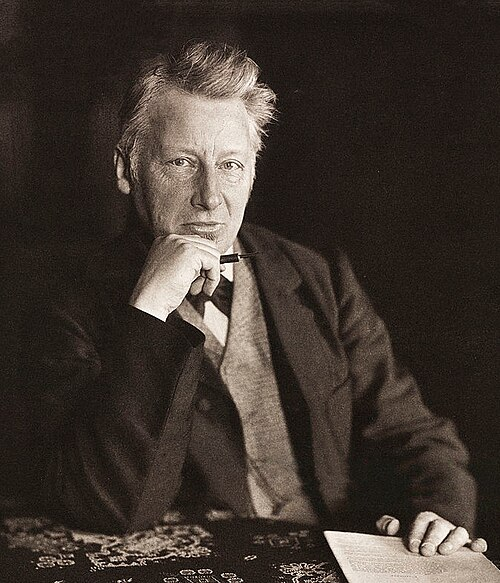
\includegraphics[width=\linewidth]{images/book3/vanthoff.jpg}
\end{minipage}\hfill
\begin{minipage}[t]{0.76\linewidth}\vspace{0pt}
Jacobus Henricus van 't Hoff (1852--1911) donna en 1884, dans ses
\emph{Études de dynamique chimique}, la relation entre la température et
la constante d'équilibre qui porte son nom, et l'année suivante la loi de la
\omterm{def:b2:chemical-potential:osmotic-pressure}{pression osmotique} du \cref{ch:b2:chemical-potential}~; dix ans plus tôt, il avait
proposé l'atome de carbone tétraédrique. Il reçut le premier prix Nobel de
chimie, en 1901. (Photographie de N. Perscheid, 1904~: domaine public,
Wikimedia Commons.)
\end{minipage}
\end{history}

\section{Variance}

Combien de grandeurs intensives un expérimentateur peut-il fixer librement avant que
l'état d'équilibre soit entièrement déterminé~?

\begin{definition}[Variance]\label{def:b2:equilibrium-shifts:variance}
Les \emph{paramètres intensifs indépendants}\index{parametre intensif independant@paramètre intensif indépendant}
d'un système à l'équilibre forment un ensemble de grandeurs intensives
(température, pression, fractions molaires dans chaque phase) que l'on peut choisir
indépendamment et qui, une fois choisies, fixent toutes les autres. Leur nombre est la
\emph{variance}\index{variance} $v$ du système.
\end{definition}

\begin{theorem}[Règle des phases]\label{thm:b2:equilibrium-shifts:phase-rule}
Pour un système de $n$ espèces réparties entre $\varphi$ phases, liées par $r$
réactions d'équilibre indépendantes et par $s$ relations supplémentaires entre
grandeurs intensives imposées par la préparation (une alimentation stœchiométrique,
l'électroneutralité),
\[
  v = c + 2 - \varphi, \qquad c = n - r - s .
\]
\end{theorem}

\begin{proof}
Variables intensives~: $T$, $p$ et, dans chaque phase, les fractions molaires des
$n$ espèces, de somme 1, soit $n - 1$ libres par phase~: en tout $2 +
\varphi(n - 1)$. Relations~: chaque espèce est en équilibre entre les
phases, soit $\varphi - 1$ égalités de \omterm{def:b2:chemical-potential:chemical-potential}{potentiels chimiques} par espèce, $n(\varphi -
1)$ en tout~; chaque réaction donne $Q = K^\circ(T)$, soit $r$ relations~; et les $s$
relations supplémentaires. Par différence~: $v = 2 + \varphi(n - 1) - n(\varphi - 1) - r -
s = n - r - s + 2 - \varphi$. (Une espèce absente d'une phase supprime à la fois une
variable et une relation.)
\end{proof}

\begin{method}[Calculer une variance]\label{met:b2:equilibrium-shifts:variance}
\begin{enumerate}
  \item Recenser les espèces avec leur phase, et compter $n$ et $\varphi$
        (chaque solide pur est une phase~; tous les gaz forment une seule phase).
  \item Compter les réactions indépendantes $r$ entre elles.
  \item Compter les relations supplémentaires $s$~: quantités en proportions stœchiométriques
        (seulement si la relation porte sur des grandeurs d'une même phase),
        électroneutralité d'une solution ionique.
  \item $v = n - r - s + 2 - \varphi$.
\end{enumerate}
\end{method}

\begin{example}[Trois variances]\label{ex:b2:equilibrium-shifts:variances}
Calcaire en récipient fermé, \ce{CaCO3(s) <=> CaO(s) + CO2(g)}~: $n = 3$, $r =
1$, $\varphi = 3$ (deux solides, un gaz)~: $v = 1$. On choisit $T$, et la pression
du dioxyde de carbone est fixée~: $p = K^\circ(T)\,p^\circ$. Un mélange gazeux de
\ce{N2}, \ce{H2} et \ce{NH3} à l'équilibre~: $n = 3$, $r = 1$, $\varphi = 1$, $v
= 3$ ($T$, $p$ et une variable de composition)~; obtenu à partir d'ammoniac seul, ou d'une
alimentation stœchiométrique, \ce{N2} et \ce{H2} sont dans le rapport 1 : 3, $s = 1$ et
$v = 2$~: à $T$ et $p$ données, la composition est fixée, ce qu'utilise le problème
du week-end.
\end{example}

\section{Déplacer un équilibre}

\begin{definition}[Déplacement d'un équilibre]\label{def:b2:equilibrium-shifts:shift}
Lorsqu'un système à l'équilibre est perturbé (variation de température, de
pression ou d'une quantité), il n'est en général plus à l'équilibre et
évolue vers un nouvel équilibre. Le \emph{déplacement de l'équilibre}\index{deplacement d'equilibre@déplacement d'équilibre}
se fait dans le sens direct si la réaction avance ($\dd\xi > 0$), dans le sens inverse
sinon.
\end{definition}

\begin{method}[Prévoir un déplacement]\label{met:b2:equilibrium-shifts:predict-shift}
Juste après la perturbation, calculer $Q$ et $K^\circ$ (ou estimer le signe de leur variation).
Si désormais $Q < K^\circ$, le déplacement se fait dans le sens direct~; si $Q > K^\circ$,
dans le sens inverse~; si l'égalité est toujours vérifiée, il n'y a pas de déplacement.
\end{method}

\begin{omfigure}
\begin{tikzpicture}[font=\small, >={Stealth}]
  \draw[->, thick] (0,0) -- (11,0) node[right] {$\ln Q$};
  \draw[omThm, thick] (5.5,0.25) -- (5.5,-0.25) node[below, align=center] {$\ln K^\circ$\\ ($= \ln Q$ avant)};
  \fill (5.5,0) circle (2pt);
  \draw[omDef, thick] (2.8,0.25) -- (2.8,-0.25) node[below] {$\ln Q$ juste après};
  \draw[->, omDef, very thick] (3.0,0.6) -- (5.2,0.6) node[midway, above] {sens direct};
  \draw[omProp, thick] (8.4,0.25) -- (8.4,-0.25) node[below] {$\ln Q$ juste après};
  \draw[->, omProp, very thick] (8.2,0.6) -- (5.8,0.6) node[midway, above] {sens inverse};
\end{tikzpicture}

{\small Une perturbation déplace $Q$ (ou $K^\circ$, si la température varie)~;
le système évolue alors jusqu'à ce que $Q = K^\circ$ de nouveau, dans le sens direct si $Q$ est devenu
trop petit, dans le sens inverse s'il est devenu trop grand.}
\end{omfigure}

\begin{proposition}[Température]\label{prop:b2:equilibrium-shifts:temperature}
À pression constante, une élévation de température déplace un équilibre dans le
sens \omterm{def:b2:reaction-enthalpy:exothermic}{endothermique} (sens direct si $\Delta_r H^\circ > 0$), une diminution dans le
sens \omterm{def:b2:reaction-enthalpy:exothermic}{exothermique}.
\end{proposition}

\begin{proof}
À composition et pression fixées, $Q$ ne varie pas avec $T$ (pour des systèmes
idéaux)~; d'après van 't Hoff, $K^\circ$ croît avec $T$ si $\Delta_r H^\circ >
0$. Juste après une élévation de $T$, on a donc $Q < K^\circ$~: sens direct.
\end{proof}

\begin{proposition}[Pression]\label{prop:b2:equilibrium-shifts:pressure}
À température et composition constantes, une augmentation de la pression totale d'un
équilibre en phase gazeuse le déplace dans le sens qui diminue le nombre de
molécules de gaz (sens direct si $\Delta\nu_{\text{gaz}} < 0$). Si $\Delta\nu_{\text{gaz}}
= 0$, la pression est sans effet.
\end{proposition}

\begin{proof}
Avec $p_i = x_ip$, $Q = \prod_i x_i^{\nu_i}\,(p/p^\circ)^{\Delta\nu_{\text{gaz}}}$~:
à composition fixée, augmenter $p$ multiplie $Q$ par
$(p'/p)^{\Delta\nu_{\text{gaz}}}$, qui est $< 1$ si $\Delta\nu_{\text{gaz}} <
0$. Alors $Q < K^\circ$~: sens direct. Les phases condensées n'interviennent pas.
\end{proof}

\begin{proposition}[Ajout d'un constituant ou d'un gaz inerte]\label{prop:b2:equilibrium-shifts:adding}
L'ajout d'une petite quantité d'un constituant gazeux $j$ à un équilibre en phase gazeuse
modifie $\ln Q$ de
\[
  \left(\frac{\partial\ln Q}{\partial n_j}\right) = \frac{\nu_j}{n_j} -
  \frac{\Delta\nu_{\text{gaz}}}{n_{\text{tot}}}\ \ \text{si sont fixés } T, p ;
  \qquad \frac{\nu_j}{n_j}\ \ \text{si sont fixés } T, V .
\]
L'ajout d'un gaz inerte est sans effet à volume constant et, à pression constante,
agit comme une diminution de la pression.
\end{proposition}

\begin{proof}
À $T$, $p$ constantes~: $Q = \prod_i n_i^{\nu_i}\,(p/(p^\circ n_{\text{tot}}))^{
\Delta\nu_{\text{gaz}}}$, dont la dérivée logarithmique par rapport à $n_j$ vaut
$\nu_j/n_j - \Delta\nu_{\text{gaz}}/n_{\text{tot}}$ (premier terme nul pour un gaz
inerte, $\nu_j = 0$). À $T$, $V$ constants~: $p_i = n_iRT/V$ et $Q = \prod_i n_i^{
\nu_i}\,(RT/(p^\circ V))^{\Delta\nu_{\text{gaz}}}$, dont la dérivée se réduit à
$\nu_j/n_j$.
\end{proof}

\begin{remark}[Un réactif ajouté qui fait reculer la réaction]\label{rem:b2:equilibrium-shifts:paradox}
Dans la synthèse de l'ammoniac, $\nu(\ce{N2}) = -1$ et $\Delta\nu_{\text{gaz}} = -2$~:
ajouter du diazote à $T$ et $p$ constantes modifie $\ln Q$ de $-1/n_{\ce{N2}} +
2/n_{\text{tot}}$, quantité positive lorsque $x(\ce{N2}) > 1/2$. Dans un mélange
déjà riche en diazote, ajouter encore du diazote dilue tant le dihydrogène
que l'ammoniac se décompose. La règle «~ajouter un réactif fait avancer la réaction~» est sûre
à volume constant, pas toujours à pression constante.
\end{remark}

\begin{proposition}[Principe de Le Chatelier]\label{prop:b2:equilibrium-shifts:le-chatelier}
Les propositions ci-dessus se résument par le \emph{principe de Le
Chatelier}\index{principe de Le Chatelier}~: un système à l'équilibre,
perturbé en température ou en pression, se déplace dans le sens qui s'oppose à
la perturbation (il absorbe de la chaleur quand on le chauffe, réduit son volume gazeux quand on le
comprime).
\end{proposition}

\begin{proof}
Il reformule la \cref{prop:b2:equilibrium-shifts:temperature} (le sens
\omterm{def:b2:reaction-enthalpy:exothermic}{endothermique} absorbe de la chaleur) et la \cref{prop:b2:equilibrium-shifts:pressure} (moins de
molécules de gaz occupent un volume plus petit à mêmes $T$ et $p$). Pour les ajouts de
matière à pression constante, le principe n'est pas fiable
(\cref{rem:b2:equilibrium-shifts:paradox})~: il faut calculer $Q$.
\end{proof}

\begin{remark}[Quand l'équilibre cesse]\label{rem:b2:equilibrium-shifts:rupture}
Un déplacement peut s'achever non par un nouvel équilibre mais par la disparition d'une phase.
Chauffé en récipient fermé, le calcaire se décompose jusqu'à ce que $p(\ce{CO2}) =
K^\circ(T)\,p^\circ$~; s'il n'y en a pas assez pour atteindre cette pression, il
disparaît entièrement et $Q$ reste inférieur à $K^\circ$~: le système est hors
d'équilibre pour de bon, comme l'avait déjà observé le volume de première année.
\end{remark}

\begin{history}[Henry Le Chatelier]
\begin{minipage}[t]{0.2\linewidth}\vspace{0pt}
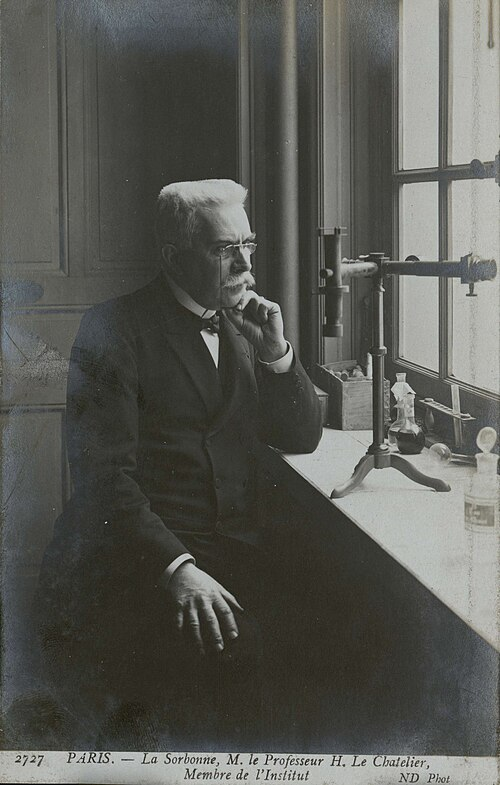
\includegraphics[width=\linewidth]{images/book3/lechatelier.jpg}
\end{minipage}\hfill
\begin{minipage}[t]{0.76\linewidth}\vspace{0pt}
Henry Le Chatelier (1850--1936), ingénieur des mines et chimiste qui travailla sur
les ciments, la métallurgie et la pyrométrie, énonça en 1884 la «~loi de \omterm{def:b2:equilibrium-shifts:shift}{déplacement
de l'équilibre}~» qui porte son nom. Il avait aussi tenté, vers 1901, de synthétiser
l'ammoniac à partir de ses éléments sous pression~; une explosion de son appareillage mit fin
à la tentative. (Photographie~: auteur inconnu, CC BY-SA 4.0, Wikimedia Commons.)
\end{minipage}
\end{history}

\section{Optimiser une synthèse}

\subsection*{L'ammoniac}

\begin{omfigure}
\begin{tikzpicture}
\begin{axis}[
  width=0.78\linewidth, height=6.2cm, xmin=500, xmax=1000, ymin=0, ymax=0.9,
  axis x line=bottom, axis y line=left, xlabel={$T$ (K)},
  ylabel={fraction molaire de \ce{NH3} à l'équilibre},
  tick label style={font=\small}, label style={font=\small}, clip=false]
\addplot[omThm, very thick] table[x=T, y=p300] {figdata/out/bachelor-2-vant-hoff-b.dat};
\addplot[omDef, very thick] table[x=T, y=p200] {figdata/out/bachelor-2-vant-hoff-b.dat};
\addplot[omProp, very thick] table[x=T, y=p50] {figdata/out/bachelor-2-vant-hoff-b.dat};
\addplot[black!60, very thick] table[x=T, y=p1] {figdata/out/bachelor-2-vant-hoff-b.dat};
\node[omThm, font=\scriptsize, anchor=south west] at (axis cs:600,0.70) {300 bar};
\node[omDef, font=\scriptsize, anchor=north east] at (axis cs:612,0.52) {200 bar};
\node[omProp, font=\scriptsize, anchor=north east] at (axis cs:578,0.30) {50 bar};
\node[black!60, font=\scriptsize, anchor=south west] (onebar) at (axis cs:520,0.13) {1 bar};
\draw[black!60] (onebar.south west) -- (axis cs:512,0.075);
\draw[dotted] (axis cs:723,0) -- (axis cs:723,0.253);
\fill[omDef] (axis cs:723,0.253) circle (1.6pt);
\end{axis}
\end{tikzpicture}

{\small Fraction molaire d'ammoniac à l'équilibre à partir d'un mélange 1 : 3 de diazote
et de dihydrogène (gaz parfaits), en fonction de la température sous quatre pressions,
calculée à partir des \omterm{def:b2:reaction-free-energy:gibbs-energy}{enthalpies libres} tabulées. La pression l'augmente, la température
la diminue~; le point marque \qty{723}{K} et \qty{200}{bar}.}
% ledger: janafG:NH3.500, janafG:NH3.600, janafG:NH3.700, janafG:NH3.800, janafG:NH3.900, janafG:NH3.1000 (computed in figdata/bachelor-2/vant-hoff.py)
\end{omfigure}

La synthèse est \omterm{def:b2:reaction-enthalpy:exothermic}{exothermique} et réduit quatre molécules de gaz à deux~: d'après
les propositions ci-dessus, une température basse et une pression élevée favorisent l'ammoniac.
Sous \qty{1}{bar} et à température ambiante, l'équilibre est presque total, mais
la réaction ne se produit pas du tout~: la triple liaison du diazote n'est rompue que
sur un catalyseur, et le catalyseur au fer n'agit qu'à plusieurs centaines de
degrés. Les usines choisissent donc~:
\begin{itemize}
  \item une température assez élevée pour la vitesse, aussi basse que le permet le catalyseur
        (vers \qty{700}{K})~;
  \item une pression élevée pour récupérer le rendement perdu à cause de la température, limitée
        par le coût de la compression et des réacteurs à parois épaisses~;
  \item une boucle~: le gaz qui sort du convertisseur est refroidi, l'ammoniac se condense
        et est extrait, et le gaz non converti est recyclé avec l'alimentation fraîche~;
        une petite \omterm{def:b2:equilibrium-shifts:single-pass}{purge} élimine l'argon et le méthane qui sinon
        s'accumuleraient.
\end{itemize}

\begin{definition}[Conversion par passage, recyclage, purge]\label{def:b2:equilibrium-shifts:single-pass}
Dans un procédé avec recyclage, la \emph{conversion par passage}\index{conversion par passage}
est la fraction d'un réactif convertie lors d'un passage dans
le réacteur~; la partie non convertie, séparée du produit, est renvoyée
à l'entrée du réacteur~: c'est le \emph{recyclage}\index{recyclage}~; une
\emph{purge}\index{purge} est un petit débit prélevé en continu sur le
recyclage pour empêcher les espèces inertes de s'accumuler.
\end{definition}

\begin{omfigure}
\begin{tikzpicture}[font=\small, >={Stealth}, box/.style={draw, thick, rounded corners=2pt, minimum width=2.1cm, minimum height=1.0cm, align=center, fill=white}]
  \node[box] (comp) at (0,0) {compresseur};
  \node[box] (conv) at (3.6,0) {convertisseur\\ (catalyseur)};
  \node[box] (cond) at (7.2,0) {refroidisseur et\\ séparateur};
  \draw[->, thick] (-3.9,0) -- (comp) node[pos=0.0, above right] {\ce{N2 + 3H2} frais};
  \draw[->, thick] (comp) -- (conv);
  \draw[->, thick] (conv) -- (cond);
  \draw[->, thick, omDef] (cond.south) -- ++(0,-1.0) node[below] {ammoniac liquide};
  \draw[->, thick, omThm] (cond.north) -- ++(0,0.9) -| (comp.north);
  \node[omThm, above] at (2.6,1.4) {recyclage (gaz non converti)};
  \draw[->, thick, black!60] (6.1,1.4) -- (6.1,2.1) node[above] {purge};
\end{tikzpicture}

{\small La boucle de l'ammoniac. Chaque passage ne convertit qu'une partie du gaz~; l'ammoniac
est condensé et extrait, et le reste est recomprimé et renvoyé avec l'alimentation
fraîche. La \omterm{def:b2:equilibrium-shifts:single-pass}{purge} empêche l'argon et le méthane, qui ne réagissent pas, de
s'accumuler.}
\end{omfigure}

\begin{history}[Haber et Bosch]
\begin{minipage}[t]{0.15\linewidth}\vspace{0pt}
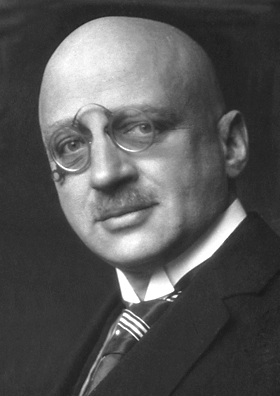
\includegraphics[width=\linewidth]{images/book3/haber.png}
\end{minipage}\hspace{0.01\linewidth}%
\begin{minipage}[t]{0.15\linewidth}\vspace{0pt}
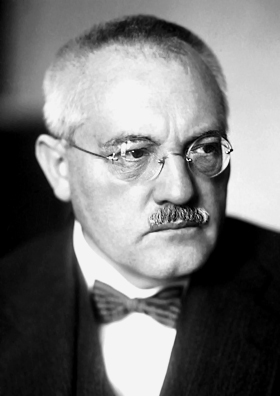
\includegraphics[width=\linewidth]{images/book3/bosch.jpg}
\end{minipage}\hfill
\begin{minipage}[t]{0.66\linewidth}\vspace{0pt}
Fritz Haber (1868--1934) mesura l'équilibre de l'ammoniac sous pression
et, en 1909, le fit produire en continu dans un convertisseur de laboratoire sur un
catalyseur à l'osmium. Carl Bosch (1874--1940) en fit une industrie, avec des
réacteurs en acier résistant au dihydrogène chaud sous pression et un catalyseur au fer
bon marché~; la première usine démarra en 1913. Haber reçut le prix Nobel en
1918, Bosch en 1931. (Portraits de la Fondation Nobel~: domaine public, Wikimedia
Commons.)
\end{minipage}
\end{history}

\subsection*{Le trioxyde de soufre}

Dans le procédé de contact, \ce{2SO2(g) + O2(g) <=> 2SO3(g)} ($\Delta_r H^\circ =
\qty{-197.8}{kJ/mol}$ pour l'équation telle qu'elle est écrite) se déroule sur un catalyseur à
l'oxyde de vanadium, actif seulement à chaud, dans plusieurs lits adiabatiques. Dans chaque lit, la
chaleur libérée élève la température, ce qui abaisse $K^\circ$~; la conversion
s'arrête quand le gaz atteint la courbe d'équilibre. Un refroidissement entre les lits le ramène
à une température où l'équilibre permet une conversion plus poussée.
% ledger: dfh:SO2_g, dfh:SO3_g

\begin{omfigure}
\begin{tikzpicture}
\begin{axis}[
  width=0.72\linewidth, height=6.4cm, xmin=600, xmax=900, ymin=0, ymax=1.08,
  axis x line=bottom, axis y line=left, xlabel={$T$ (K)},
  ylabel={conversion de \ce{SO2}}, tick label style={font=\small},
  label style={font=\small}, clip=false]
\addplot[black, very thick] table[x=T, y=X] {figdata/out/bachelor-2-vant-hoff-c.dat};
\addplot[omThm, thick] table[x=T, y=X] {figdata/out/bachelor-2-vant-hoff-bed1.dat};
\addplot[omThm, thick] table[x=T, y=X] {figdata/out/bachelor-2-vant-hoff-bed2.dat};
\addplot[omThm, thick] table[x=T, y=X] {figdata/out/bachelor-2-vant-hoff-bed3.dat};
\draw[->, omDef, thick] (axis cs:892.8,0.676) -- (axis cs:712,0.676);
\draw[->, omDef, thick] (axis cs:784.4,0.924) -- (axis cs:712,0.924);
\node[font=\scriptsize, anchor=south west] at (axis cs:860,0.84) {équilibre};
\node[omThm, font=\scriptsize, anchor=west] at (axis cs:800,0.24) {lit 1 (adiabatique)};
\node[omDef, font=\scriptsize, anchor=south] at (axis cs:800,0.68) {refroidissement};
\end{axis}
\end{tikzpicture}

{\small Conversion d'équilibre de \ce{SO2} en \ce{SO3} en fonction de la température
(en noir) pour une alimentation modèle à \qty{10}{\percent} de \ce{SO2} et \qty{11}{\percent}
de \ce{O2} sous \qty{1}{bar}, et chemin du gaz à travers trois lits adiabatiques
(en rouge, la température montant à mesure que la réaction chauffe le gaz), refroidi entre les
lits (en bleu).}
% ledger: janafG:SO2.600, janafG:SO2.700, janafG:SO2.800, janafG:SO2.900, janafG:SO3.600, janafG:SO3.700, janafG:SO3.800, janafG:SO3.900 (computed in figdata/bachelor-2/vant-hoff.py; feed and adiabatic rise are model values)
\end{omfigure}

\section{Exercices}

\begin{exercise}[$\star$]\label{exo:b2:equilibrium-shifts:1}
Calculer $K^\circ$ à \qty{298}{K} pour une réaction de $\Delta_r G^\circ =
\qty{-32.8}{kJ/mol}$, puis pour $\Delta_r G^\circ = \qty{+32.8}{kJ/mol}$.
Quelle variation de $\Delta_r G^\circ$ multiplie $K^\circ$ par 100~?
\end{exercise}

\begin{exercise}[$\star$]\label{exo:b2:equilibrium-shifts:2}
Pour la synthèse de l'ammoniac, $K^\circ(298) = \num{5.4e5}$ et $\Delta_r H^\circ =
\qty{-91.9}{kJ/mol}$. Estimer $K^\circ$ à \qty{400}{K} à l'aide de la \omterm{thm:b2:equilibrium-shifts:vant-hoff}{relation de
van 't Hoff} intégrée~; les tables donnent 35.6.
\end{exercise}

\begin{exercise}[$\star$]\label{exo:b2:equilibrium-shifts:3}
Calculer la \omterm{def:b2:equilibrium-shifts:variance}{variance} de~: (a) l'eau liquide en équilibre avec sa vapeur~;
(b) \ce{CaCO3(s) <=> CaO(s) + CO2(g)} en récipient fermé~; (c) \ce{N2},
\ce{H2}, \ce{NH3} à l'équilibre, alimentation quelconque~; (d) \ce{C(s) + H2O(g) <=>
CO(g) + H2(g)}.
\end{exercise}

\begin{exercise}[$\star$]\label{exo:b2:equilibrium-shifts:4}
Pour \ce{N2O4(g) <=> 2NO2(g)}, $\Delta_r H^\circ > 0$. Dans quel sens
l'équilibre est-il déplacé par un chauffage à pression constante, par une compression à
température constante, par un ajout d'argon à volume constant~?
\end{exercise}

\begin{exercise}[$\star\star$]\label{exo:b2:equilibrium-shifts:5}
Pour \ce{N2(g) + O2(g) <=> 2NO(g)}, $\Delta_r H^\circ = \qty{180.6}{kJ/mol}$,
$\Delta_r S^\circ = \qty{24.8}{J/(K.mol)}$. Calculer $K^\circ$ à \qty{298}{K}
et à \qty{2000}{K} (\omterm{def:b2:reaction-free-energy:ellingham-approximation}{approximation d'Ellingham}), ainsi que la fraction molaire de
\ce{NO} dans l'air ($x(\ce{N2}) = 0.78$, $x(\ce{O2}) = 0.21$, peu consommés) à
l'équilibre à \qty{2000}{K}. Pourquoi les moteurs produisent-ils ce polluant, et pourquoi
subsiste-t-il dans les gaz d'échappement refroidis~?
\end{exercise}

\begin{exercise}[$\star\star$]\label{exo:b2:equilibrium-shifts:6}
Une estérification $\mathrm{A + B \rightleftharpoons E + W}$ en phase liquide
a pour $K^\circ = 4.0$ (activités assimilées aux fractions molaires). À partir de
\qty{1.0}{mol} d'acide A, calculer la quantité d'ester obtenue avec \qty{1.0}{mol}, puis
\qty{3.0}{mol} d'alcool B. Expliquer, à l'aide de $Q$ et de $K^\circ$, pourquoi éliminer
l'eau au fur et à mesure de sa formation rend la réaction totale.
\end{exercise}

\begin{exercise}[$\star\star$]\label{exo:b2:equilibrium-shifts:7}
À \qty{298}{K} et sous \qty{1}{bar}, $K^\circ = 0.148$ pour \ce{N2O4 <=> 2NO2}.
Calculer le coefficient de dissociation de \qty{1}{mol} de \ce{N2O4}. On ajoute ensuite
\qty{1}{mol} d'argon à pression totale constante~: calculer le nouveau
coefficient de dissociation, et expliquer. Que se passe-t-il si l'argon est ajouté à
volume constant~?
\end{exercise}

\begin{exercise}[$\star\star$]\label{exo:b2:equilibrium-shifts:8}
Le chlorure d'ammonium se sublime en se dissociant, \ce{NH4Cl(s) <=> NH3(g) +
HCl(g)}. Calculer la \omterm{def:b2:equilibrium-shifts:variance}{variance} lorsque le gaz provient uniquement du solide, puis lorsque
l'on a ajouté un peu d'ammoniac. Que signifie chaque cas pour l'expérimentateur~?
\end{exercise}

\begin{exercise}[$\star\star$]\label{exo:b2:equilibrium-shifts:9}
Les tables donnent, pour la synthèse de l'ammoniac, $K^\circ = 0.0993$ à \qty{500}{K} et
$K^\circ = \num{1.72e-3}$ à \qty{600}{K}. En déduire $\Delta_r H^\circ$ sur cet
intervalle et comparer à sa valeur à \qty{298}{K}.
\end{exercise}

\begin{exercise}[$\star\star\star$]\label{exo:b2:equilibrium-shifts:10}
Démontrer le contre-exemple de la \cref{rem:b2:equilibrium-shifts:paradox}~: écrire
le $Q$ de la synthèse de l'ammoniac avec les quantités et la pression totale, calculer
$\partial\ln Q/\partial n(\ce{N2})$ à $T$ et $p$ constantes, et trouver la
condition sur $x(\ce{N2})$ pour laquelle l'ajout de diazote déplace l'équilibre
dans le sens inverse. La même chose peut-elle se produire à volume constant~?
\end{exercise}

\begin{exercise}[$\star\star\star$]\label{exo:b2:equilibrium-shifts:11}
Du calcaire est chauffé à \qty{1100}{K} dans un récipient fermé initialement vide de
\qty{10.0}{L}, où $\Delta_r G^\circ = \qty{1.62}{kJ/mol}$ pour sa
décomposition (\cref{ch:b2:reaction-free-energy}). Calculer $K^\circ$ et la
pression d'équilibre du dioxyde de carbone. Déterminer l'état final pour
\qty{0.050}{mol} puis pour \qty{0.200}{mol} de calcaire.
\end{exercise}

\begin{exercise}[$\star\star\star$]\label{exo:b2:equilibrium-shifts:12}
Lire sur la figure du procédé de contact la conversion et la température à la
sortie de chaque lit. Expliquer pourquoi un seul lit adiabatique, si long soit-il, ne pourrait
dépasser environ 68\,\% de conversion avec cette alimentation, pourquoi on refroidit le gaz
entre les lits plutôt que de maintenir le catalyseur froid tout du long, et ce qui limite
la conversion du dernier lit.
\end{exercise}

\section{Problème~: la boucle de l'ammoniac}

\begin{problem}[{Problème du week-end --- la constante d'équilibre de la synthèse
de l'ammoniac et sa dépendance en température, la composition dans les conditions du
convertisseur, les déplacements dus à la pression, à la température et aux gaz inertes, et
la boucle}]
\label{pb:b2:equilibrium-shifts:1}
L'ammoniac est produit par \ce{N2(g) + 3H2(g) <=> 2NH3(g)} à partir d'une alimentation stœchiométrique.
Données~: à \qty{298.15}{K}, $\Delta_f H^\circ(\ce{NH3}) = \qty{-45.94}{kJ/mol}$,
$S^\circ_m$ (\unit{J/(K.mol)}) \ce{NH3} 192.77, \ce{N2} 191.61, \ce{H2} 130.68~;
les tables donnent $\Delta_f G^\circ(\ce{NH3}) = \qty{+27.19}{kJ/mol}$ à
\qty{700}{K} et \qty{+38.66}{kJ/mol} à \qty{800}{K}. Les gaz sont parfaits~;
$R = \qty{8.314}{J/(K.mol)}$.
% ledger: dfh:NH3_g, s0:NH3_g, s0:N2_g, s0:H2_g, janafG:NH3.700, janafG:NH3.800

\medskip
\noindent\textbf{Partie I --- La constante.}
\begin{enumerate}
  \item Calculer $\Delta_r H^\circ$, $\Delta_r S^\circ$ et $\Delta_r G^\circ$ à
        \qty{298}{K}, ainsi que $K^\circ(298)$.
  \item Calculer $K^\circ$ à \qty{700}{K} et à \qty{800}{K} à partir des tables.
  \item En déduire, à partir de ces deux valeurs, le $\Delta_r H^\circ$ moyen entre
        \qty{700}{K} et \qty{800}{K}, et comparer à la question 1.
  \item Estimer $K^\circ(\qty{723}{K})$ à partir des deux valeurs tabulées à l'aide de
        la \omterm{thm:b2:equilibrium-shifts:vant-hoff}{relation de van 't Hoff}.
  \item Calculer $K^\circ(\qty{723}{K})$ dans l'\omterm{def:b2:reaction-free-energy:ellingham-approximation}{approximation d'Ellingham} à partir
        des données à \qty{298}{K}, et commenter l'écart.
\end{enumerate}

\medskip
\noindent\textbf{Partie II --- L'équilibre dans le convertisseur.}
\begin{enumerate}[resume]
  \item À partir d'une alimentation de \qty{1}{mol} de \ce{N2} et \qty{3}{mol} de \ce{H2}, écrire les
        quantités à l'avancement $\xi$ et la quantité totale.
  \item Montrer que, $x$ désignant la fraction molaire d'ammoniac, les fractions molaires
        de \ce{N2} et de \ce{H2} valent $(1-x)/4$ et $3(1-x)/4$.
  \item Montrer que $\dfrac{x}{(1-x)^2} = \dfrac{\sqrt{27}}{16}\,\dfrac{p}{p^\circ}\,
        \sqrt{K^\circ}$.
  \item Calculer $x$ à \qty{723}{K} et sous \qty{1}{bar}.
  \item Calculer $x$ à \qty{723}{K} et sous \qty{200}{bar}.
  \item Calculer la \omterm{def:b2:equilibrium-shifts:variance}{variance} du système et expliquer pourquoi $T$ et $p$ fixent la
        composition.
\end{enumerate}

\medskip
\noindent\textbf{Partie III --- Déplacements.}
\begin{enumerate}[resume]
  \item Sans calcul, dans quel sens l'équilibre se déplace-t-il lorsque
        la pression augmente~? Lorsque la température augmente~?
  \item De l'argon entre avec l'air utilisé pour produire le diazote. À pression totale
        constante, comment sa présence déplace-t-elle l'équilibre~?
  \item Un mélange à l'équilibre a $x(\ce{N2}) = 0.30$. L'ajout d'un peu de
        diazote à $T$ et $p$ constantes le déplace-t-il dans le sens direct ou inverse~?
  \item La réponse changerait-elle à volume constant~?
  \item Avant que le gaz ne retourne au convertisseur, on en condense
        l'ammoniac. Quel est l'effet sur $Q$ à l'entrée du convertisseur~?
\end{enumerate}

\medskip
\noindent\textbf{Partie IV --- La boucle.}
\begin{enumerate}[resume]
  \item Le gaz sort du convertisseur avec \qty{18}{\percent} d'ammoniac, au-dessous de
        la valeur d'équilibre. Pourquoi un convertisseur réel n'atteint-il pas
        l'équilibre~?
  \item Calculer la \omterm{def:b2:equilibrium-shifts:single-pass}{conversion par passage} du dihydrogène correspondant à
        $x(\ce{NH3}) = 0.18$ pour une alimentation stœchiométrique.
  \item Le gaz non converti est recyclé. En régime permanent, \qty{1.00}{mol}
        de \ce{N2} frais entre par unité de temps~: quelle quantité d'ammoniac sort, et quelle
        quantité de diazote traverse le convertisseur par unité de temps~?
  \item Pourquoi faut-il purger un peu de gaz du \omterm{def:b2:equilibrium-shifts:single-pass}{recyclage}~?
  \item Pourquoi ne fait-on pas fonctionner le convertisseur à \qty{500}{K}, où l'équilibre est
        bien plus favorable~?
  \item Donner la fraction molaire d'ammoniac à l'équilibre à \qty{723}{K} et sous
        \qty{200}{bar} pour une alimentation stœchiométrique, dans le modèle des gaz parfaits.
\end{enumerate}
\end{problem}
